% !TEX root = UsevichGDRISIS2020.tex
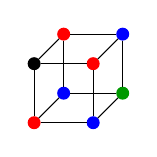
\begin{tikzpicture}
\tikzstyle{p3} = [color = green!60!black]
\tikzstyle{p2} = [color = blue]
\tikzstyle{p1} = [color = red]
\tikzstyle{p0} = [color = black]

\begin{scope}[xscale= 0.75,yscale=0.75]
\tikzstyle{dot} = [draw,circle,minimum size=1.5mm,fill,inner sep=0mm]

\draw(0,0) node[dot,p1]          (v0001) {};
\draw(1,0) node[dot,p2]          (v0011) {};
\draw(0,1) node[dot,p0]          (v0000) {};
\draw(1,1) node[dot,p1]          (v0010) {};
\draw(0.5,0.5) node[dot,p2]      (v0101) {};
\draw(1.5,0.5) node[dot,p3]      (v0111) {};
\draw(0.5,1.5) node[dot,p1]      (v0100) {};
\draw(1.5,1.5) node[dot,p2]      (v0110) {};

\draw (v0000) -- (v0010) -- (v0011) -- (v0001) -- (v0000);
\draw (v0100) -- (v0110) -- (v0111) -- (v0101) -- (v0100);
\draw (v0000) -- (v0100);
\draw (v0010) -- (v0110) ;
\draw (v0001) -- (v0101);
\draw (v0011) -- (v0111) ;

\end{scope}
\end{tikzpicture}